\renewcommand\evenpagerightmark{{\scshape\small Scale-up}}
\chapter[Scale-up]%
{Scale-up}
\label{Scale-up}

\section{The geometry}
\subsection{What is required}

The main objective of this burner is to investigate the effect of swirl on diffusion flame in an oxycombustion with a coaxial shape. The  work on ATR30 burner has been to establish a similar environment as the Freiberg OPTISOS study (in terms of flame topology ) with scale-up rules : conservation of geometry, speeds, swirl, $Z_{st}$, $J$. The aim of this burner is to be studied in a very similar environment as the study on ATR30 burner. Consequently, though the geometry is to evolve, a particular care is paid so that the speeds and the mass flows remain constant.

Let us make a bill of specifications for that burner :
\begin{enumerate}
\item The Swirl number must be modular from 0 to 2 (margins included)
\item The outlet speeds must be the same as the OPTYSOS study
\item The mass flows have to be similar to the Calhory sizing study with ATR30 burner
\item The internal axial swirled pipe will be the same as the ATR30 burner (since it is already crafted)
\item The H20 intermediate injection will not be used
\item The geometry must be convenient with combustion (in particular, the wall between the fuel and the oxidant must not exceed $1-2mm$)  
\item The shape must be as simple as possible
\end{enumerate}
One must acknowledge that these objectives do not seem so ambitious, but the following study enhances the difficulties.

\begin{figure}[h!]
  \centering
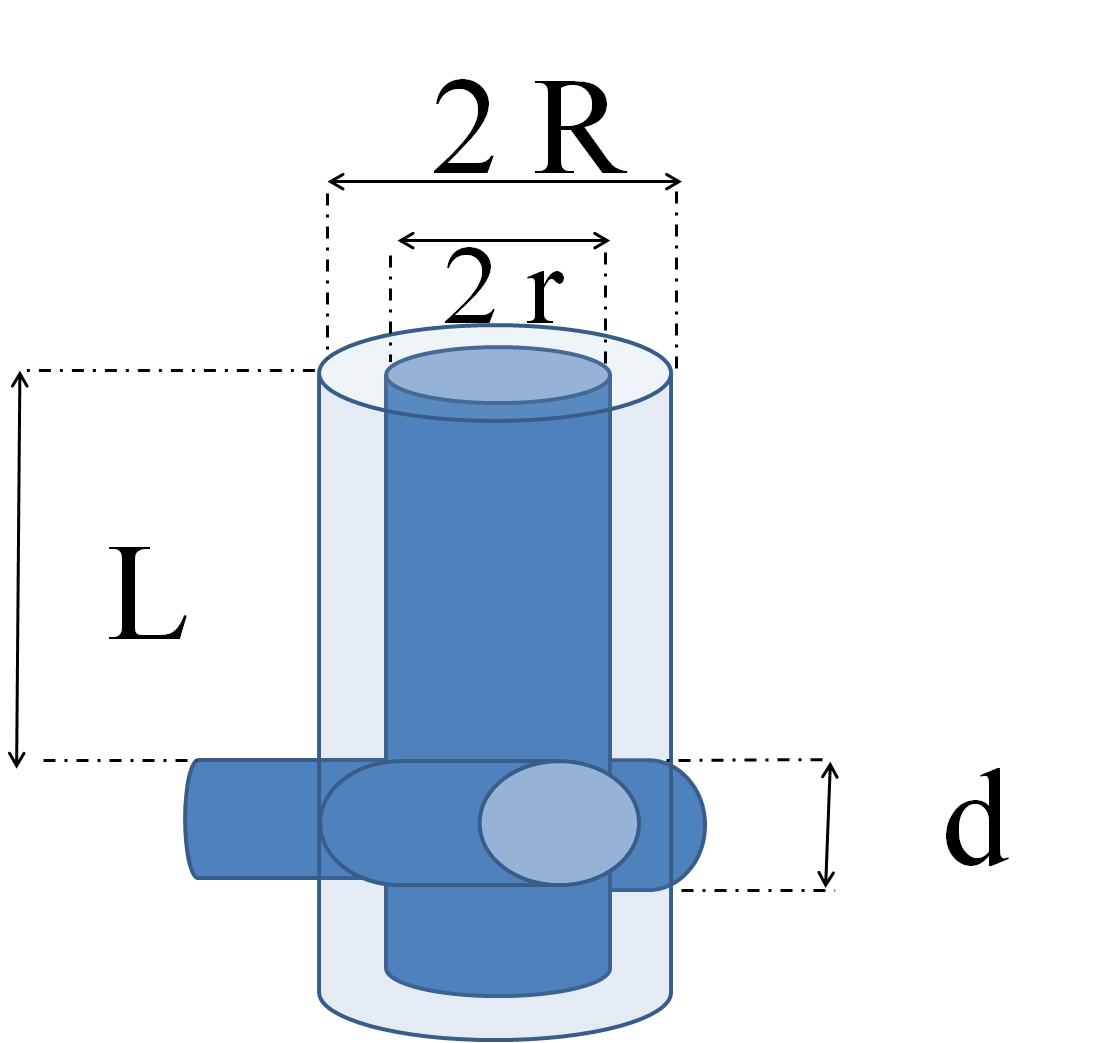
\includegraphics[width=0.45\textwidth]{fig/proto.png}
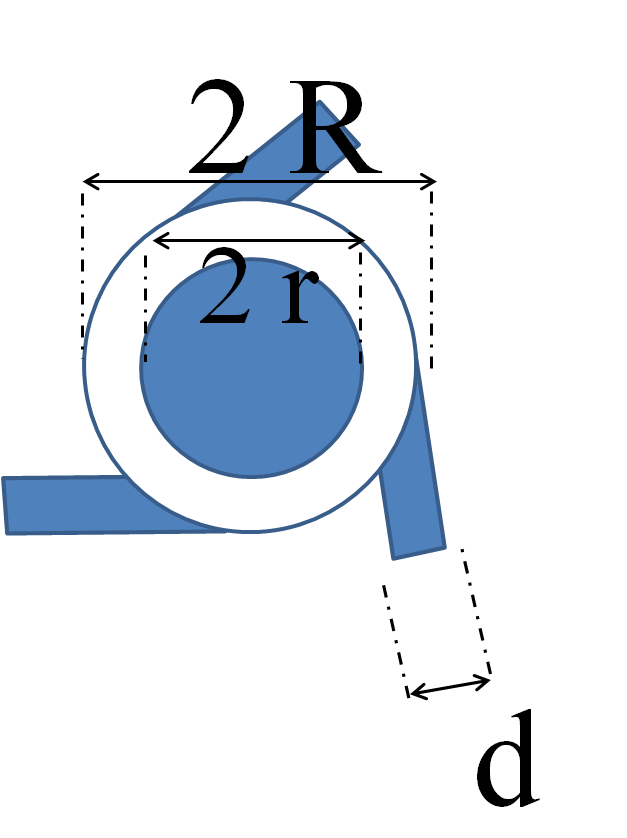
\includegraphics[width=0.45\textwidth]{fig/proto_dessus.png}
  \caption{Notations and hypothetical geometry of the prototype burner}
 \label{proto}
\end{figure}
Figure \ref{proto} gives the geometrical notations. Only the outer flow is studied, since the internal pipe is the pipe of the ATR30_norm, whose geometry and swirl are already given.

Let us call $U_{out}$ the speed at the outlet of the outer pipe (at the top of the figure), $U_{in}$ the speed at the inlet of the outer pipe and $W$ the speed in the tangential pipes.

The mass conservation gives :

$\dot{m_{in}}+\dot{m_{tangential}}=\dot{m_{out}}$

The fluid being the same in the axial and the tangential injections, we have :
$U_{in}+W \frac{A_{\theta}}{A_{z}}=U_{out}$ 

\subsection{The problem of tangential speed}

In this section, it is demonstrated that the geometrical area providing the tangential injections needs to be as big as possible.

Let us consider the case where the swirl is maximum, so the mass flow entirely comes from the tangential injections, and the injected axial flow is null. Then the mass conservation gives :

$W \frac{A_{\theta}}{A_{z}}=U_{out}$ 

For practical reasons, $W$ is required smaller than $100m/s$. $U_{out}$ is the speed we want to fit to Optysos study, so it is fixed to $U_{out}=75m/s$. 

\subsection{First try with circular pipes injections}

It is demonstrated that the pipe geometry for the tangential injections seems not a good solution.

If the axial pipe goes from $r$ to $R$, there is only the room $d=R-r$ to put a circular pipe of diameter $d$ between the boundaries of the axial pipe.
If we compute the ratio :
$ \frac{A_{\theta}}{A_{z}}=\frac{N\pi d^2/4}{\pi (R^2-r^2)}$ , N being the number of tangential injections

Then, we  have :

$ \frac{A_{\theta}}{A_{z}}=\frac{N(R-r)}{4 (R+r)}$
 since $r$ is fixed to $7.05mm$, we see that we need $R$ big and $N>4$  so that $W<75m/s$.
 
 This is impossible to achieve. The first conclusion is that it using pipes for tangential injections as it is the case in fig \ref{proto} will give too big tangential speeds.
 
 \subsection{Paralepipedic injections }

Let us now consider that there are $N$ injections of paralepipedic pipes, of diameter $d$ and height $H$.



